\chapter{Estado del arte}
\label{chap:estado del arte}

Actualmente existen diversos tipos de herramientas que realizan tareas de recolección, filtrado y gestión de eventos dentro un sistema. Las que se han podido analizar y comprobar han sido las siguientes:

\section{Lookwise}
\hspace*{1.7in}{
\includegraphics[scale=0.5]{diagramas/lookwise-logo.png}}

Lookwise es una herramienta corporativa que hace las funciones de SIEM en materia de gestión de seguridad, Big Data y cumplimiento normativo (ISO/LOPD).

\subsection{Características}

Gestión centralizada
\begin{itemize}
\item Interfaz gráfica de administración y operación centralizada.
\item Creación y distribución de políticas de forma remota.
\item Integración de alertas y explotación de resultados.
\item Cuadro de mandos de seguridad.
\item Visibilidad en base a roles y permisos.
\item Integración con sistemas SIEM.
\end{itemize}

Comunicaciones
\begin{itemize}
\item Autenticadas y cifradas
\item Ininterrumpidas
\item Comprimidas
\end{itemize}

Plataformas soportadas
\begin{itemize}
\item Familia Windows XP (Windows Kernel 5)
\item Familia Windows 7 (Windows Kernel 6)
\end{itemize}

Arquitectura
\begin{itemize}
\item Arquitectura Distribuida.
\item Arquitectura Modular.
\item Flexible y escalable.
\item Balanceo de carga.
\item Despliegue remoto de funcionalidades y actualizaciones.
\end{itemize}

\hspace*{-0.25in}{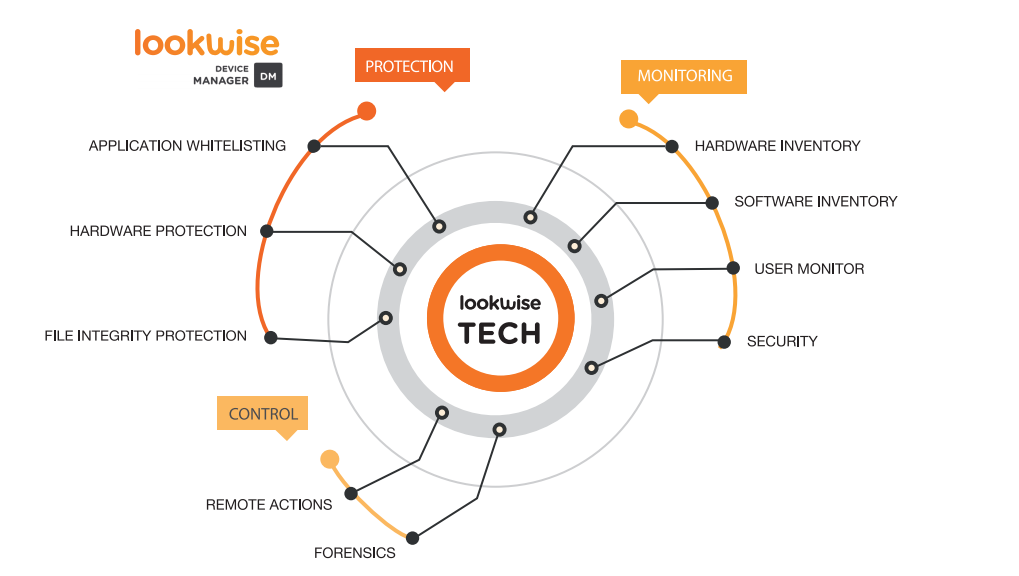
\includegraphics[scale=0.5]{diagramas/funcionalidades-lookwise.png}}

\subsection{Análisis de la herramienta}

La herramienta de análisis de incidencias y vulnerabilidades hace la mismas funcionalidades de un SIEM pero con una capa más enfocada a sistemas PCI y de infraestructuras críticas. Gestiona eventos del sistema y los correla con alertas predefinidas internamente o que se hayan incluido cómo especificación del cliente. Detecta fallos en el Active Directory y nos genera un sistema de informe con las incidencias más graves de cara a la parte de consultoría de incidentes por parte el equipo interno.


\section{ELK Stack}

La pila ELK se basa en una solución open-source de tres productos bien diferenciados que se relacionan entre sí de la siguiente manera:

\hspace*{.5in}{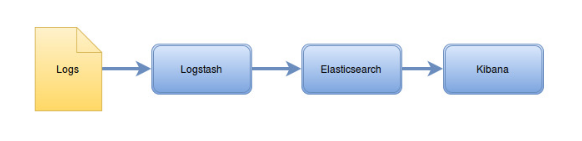
\includegraphics[scale=0.65]{diagramas/elk-stack.png}\\}

\begin{itemize}
\item Elasticsearch para la búsqueda de datos y análisis en profundidad de un sistema.
\item Logstash para el registro centralizado de logs y su posterior normalización y enriquecimiento de datos.
\item Kibana cómo herramienta de visualización de los datos recolectados y procesados anteriormente según las especificaciones que queramos para el filtrado.
\end{itemize}

\subsection{Elasticsearch}
\hspace*{2in}{
\includegraphics[scale=0.15]{diagramas/elasticsearch-logo.png}\\}
Elasticsearch es un motor open-source de búsqueda y análisis de información de gran escalabilidad. Esta herramienta permite almacenar, buscar y analizar grandes volúmenes de datos de forma rápida y en tiempo real. Se suele utilizar cómo motor/tecnología subyacente de otras aplicaciones (wrapers), permitiendo así realizar funciones de búsqueda complejas de una manera más ágil.\\

\subsection{Logstash}
\hspace*{1.75in}{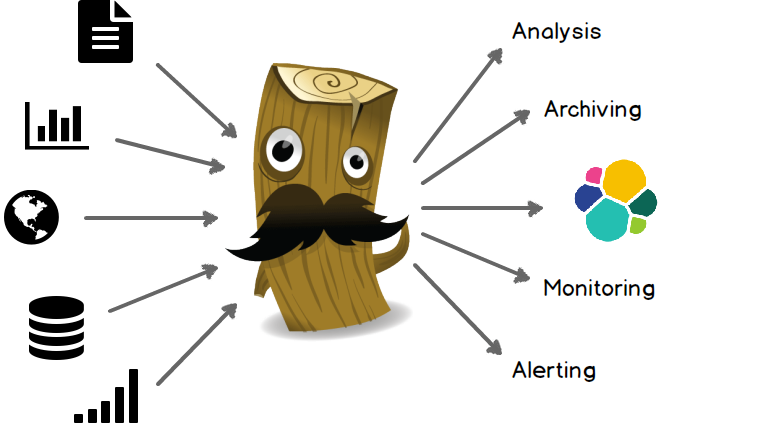
\includegraphics[scale=0.25]{diagramas/logstash.png}\\}
Logstash es un motor open-source de recopilación de datos con capacidad de multihebrado en tiempo real. Esta herramienta puede unificar dinámicamente datos de diferentes fuentes y normalizar dichos datos para los outputs de nuestra elección. Además nos permite filtrar y discretizar todo los datos recolectados para obtener información analítica que pueda ser visualizada.\\

\hspace*{.5in}{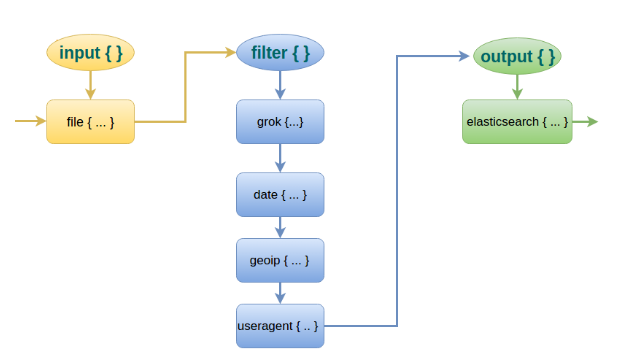
\includegraphics[scale=0.65]{diagramas/logstash-configuration.png}\\}

Con logstash, cualquier tipo de evento puede ser enriquecido y transformado con un amplio repertorio de inputs/filtros y los datos de salida, se pueden modificar dependiendo del tipo de software sobre el que queramos introducir esos datos (plugins y códecs).\\

\subsection{Kibana}
\hspace*{2.25in}{
\includegraphics[scale=0.75]{diagramas/kibana-logo.png}\\}
Kibana es una plataforma open-source de análisis y visualización de datos diseñada para trabajar con Elasticsearch. Kibana se utiliza para para buscar, ver e interactuar con datos almacenados en los índices o base de datos de Elasticsearch. De esta forma se puede realizar fácilmente un análisis avanzado de datos que permita visualizarlo en una gran variedad de gráficas, tablas y mapas.\\

Kibana hace que sea fácil de entender y procesar grandes volúmenes de datos. Mediante su interfaz basada en un cliente web, nos permite crear de forma simple y ágil filtros sobre los datos extraidos mediante consultas a la bd de Elasticsearch en tiempo real.\\


\subsection{Análisis de la herramienta}

La pila ELK, cómo bien se ha comentado en los tres puntos anteriores nos permite recolectar, procesar y correlar cualquier tipo de logs que genere nuestro sistema de una manera visual, ágil y fácil de entender. \\

El motor de indexación de datos, Elasticsearch, nos permite obtener una ejecución en tiempo real de los logs del sistema así cómo poder escalar dicho volumen de datos dependiendo de la situación. El único inconveniente que podría sacar de este fragmento de la pila es que el sistema de referenciación de documentos internos es mediante json. Es un formato muy versátil pero incapaz de tener funcionalidad por si sola.\\

Después tenemos Logstash que es el encargado de hacer de middleware entre elastic y kibana, es decir, la parte de la recogida de muestras/eventos y la parte dónde se visualizan esas muestras. Logstash hace de filtro y de motor de normalización de datos entre los diferentes activos que tiene asignados para así poder tener todos los datos unificados según la especificación que queramos dar a cada uno de ellos. \\

Cada parte de la pila esta desarrollada en su propio lenguaje de desarrollo, siendo Java (o Groovy) el lenguaje de desarrollo de elastic, Ruby el de logstash y Javascript para Kibana. El único inconveniente que se ha podido observar es que la solución ELK está diseñada para trabajar más optimizada en entornos de cloud computing y no de manera local en un servidor. Dado que tendría que usar recursos propios de la máquina y conforme se vayan escalando nuevo recursos estos irán aumentando los de la máquina. Si hay limitación de hardware por los mismo puede llegarse a experimentar un cuello de botella entre elastic y kibana, siendo la carga de datos muy lenta y con tiempos de refresco bastante altos. \\

\section[SIEM]{Sistemas de recolección y administración de eventos: SIEM}

Un sistema de recolección y administración de eventos (SIEM), es una tecnología que se usa para la detección de amenazas y respuesta ante incidentes de seguridad a través de la obtención, en tiempo real o mediante un histórico, de eventos de seguridad a partir de una amplia variedad de fuentes o activos. Una de las principales características de un SIEM, es el gran alcance que tiene a la hora de recopilar una gran cantidad eventos para posteriormente correlar dichos eventos con alertas o incidencias de seguridad conocidas dentro del entorno corporativo.\\

\subsection{Principales características}

Estos son los puntos que principalmente gestiona un SIEM:\\

\begin{itemize}
\item Gestión de parches (actualizaciones) del kernel o software de terceros cómo adobe, java, etc.
\item Antivirus en máquinas de usuarios o en servidor.
\item Gestión de cortafuegos.
\item Integración con Active Directory (LDAP).
\item Sistema de prevención de intrusiones (en red: NIPS / basado en hosts: HIPS)
\item Proxy / Filtro de contenidos
\item Email: anti-spam / anti-phishing
\item Análisis de vulnerabilidades
\item Herramientas de seguridad opcionales:
  \begin{itemize}
  \item IPS para redes Wifi.
  \item Control de firewall web.
  \item Aplicaciones que monitoricen bases de datos.
  \item Prevención de pérdida de datos.
  \item Gestión de riesgos y herramienta de cumplimiento de políticas
  \end{itemize}
\end{itemize}

\subsection{Análisis}

Aunque esta herramienta sea cómo un conglomerado de aplicaciones o herramientas de detección y análisis, su puesta en marcha no es así tan fácil cómo cabría esperarse dado que cada despliegue requiere de unos activos o fuentes diferentes. Además, cada solución final requerirá de unas especificaciones distintas, con lo que su implantación depende en gran medida de la facilidad de adaptación al entorno y también de que los responsables de dicha herramienta tengan un profundo conocimiento sobre ella.\\

Una de las palabras más comunes que definen la implementación de un SIEM es: desalentador. A menudo termina costando más de lo previsto, requiere una experiencia sobre la herramienta que a menudo suele ser externalizada (sobre el propio fabricante) y puede llevar un tiempo considerable antes de obtener resultados tangibles.\\

Los motivos para los que generalmente se introducen un sistema cómo un SIEM en la red corporativa suelen ser varios, pero entre los más destacados suelen ser: el cumplimiento de una normativa industrial o de un gobierno, la gestión de incidentes recurrentes de seguridad o también que en la licitación de un contrato esté contemplado la puesta en marcha de este sistema para una mayor calidad del servicio prestado por un tercero o por la propia entidad. Y aún así, que la propia empresa ya gestione sus eventos internos o los monitorice, no implica que su migración al SIEM sea inmediata.\\

Además, la licitación o adquisición de un producto de estas características supone que el entorno sobre el que se va a aplicar contiene dispositivos de seguridad que monitorizar (sino se está realizando dicho control), que se dispongan de herramienta de centralización de datos (físicamente o en cloud) y que se quiera un sistema de gestión 24/7, incluido la monitorización fuera de horario laboral.\\

Son estas razones por las que a veces un sistema tan complejo y gigantesco puede que genere un sobrecoste o cubra pocas áreas de la red en las que no se tiene necesidad de vigilar. Siendo esto un incoveniente finalmente, dado que hay otras herramientas (de las que se nutre el SIEM) que ya cumplen con dicha funcionalidad a coste de tener un sistema muy pesado que gestionar.\\

--------------------------------------------------

\section{Solución tecnológica de mi proyecto}

La idea principal de mi proyecto surge fruto de la necesidad de monitorizar un red corporativa a través de un mecanismo de gestión automatizada de eventos, o lo que viene siendo un SIEM. Los pasos para la realización de este sistema se han modularizado y dividido en diferentes etapas que se acometarán cómo un todo dentro de un proyecto de investigación del grupo de ciberseguridad de la universidad de granada (UCyS - \url{http://ucys.ugr.es/}).\\

Dicho proyecto consistirá en la monitorización de la red corporativa de Mercagranada y todo lo que ello conlleva: sistemas informáticos, gestión de bases de datos, sistemas pci, sistemas perimetrales, etc. \\

[Explicar que es lo que diferencia mi pfc de las anteriores herramientas analizadas: lookwise, ELK y un SIEM. Hay otras herramientas cómo splunk o sumologic - \url{http://blog.takipi.com/log-management-tools-face-off-splunk-vs-logstash-vs-sumo-logic/}]

\section{Tecnologías implementadas}

A continuación explicaré las diferentes tecnologías/bibliotecas/lenguajes que se han empleado para la elaboración del proyecto y porque se han escogido por encima de otras posibles soluciones.

\subsection{Python}




python
django
paquetes python con el requirements
d3
c3
latex
react
sqlite
rsyslog
logrotate
syslog
iptables
django-rest
json
pycharm
taiga
bitbucket
git
digitalocean
nginx


python: librerias cómo pygtail, gunicorn, django (framework), d3, c3, react
